\section*{Results}
\label{results}
We apply our \minapproxdesc{} approach on the Influenza incidence data from the CDC.
We explore the quality of descriptions, the effects of parameters, including 
relaxed versions, and with negative clauses. We discuss our ranking approach,
and some of the trends and surprises we find. 

\subsection*{ Description of Dataset}
We use the incidence data from CDC to prepare a dataset for any given week.  In our experiments, we use data corresponding to weeks for the years 2014 to 2017. The dataset for any week has the following size:

1. Number of regions (states) or rows: 51 (50 states and District of Columbia) 

2. Number of features or columns :  42 (spatial, temporal, and severity features)

Therefore, the data matrix $D$ for a week has 2142 entries. 

The features can be categorized as follows:

1. \textbf{Geographical/ Spatial} :  Features such as Great Lakes, South East, Mid-Atlantic etc. %The set of states that have such a feature is static over time. 

2. \textbf{Temporal}: Features such as Was1_high, Was2_moderate, Was52_high, etc. %The elements in the set of states that have such a feature vary over time. 

%A fixed number of states have the spatial features such as regions of US like Great Lakes, South East, Mid-Atlantic, etc. However,  varying set of states could have the temporal features such as states with high activity a week ago (Was1_high), states with moderate activity a year ago (Was52_moderate), etc., depending on the year and week of our interest. 

For each experiment discussed below, our algorithm ran within a few seconds.

%%We discuss three types of results, which illustrate the kinds of insights
%%that can be derived.
%%\begin{enumerate}
%%\item 
%%\emph{Succinct representations for sets having specific characteristics}:
%%an example of this is the set of states with high activity during a week as the target set.
%%We find that our approach often gives succinct representations and new insights into
%%the structure of such sets. We find that in many cases, the relaxed version,
%%i.e., with $\gamma>0$, has a more succinct and intuitive description.
%%Similarly, allowing negative clauses also leads to better descriptions in some cases.
%%\item 
%%\emph{Interesting temporal trends}: 
%%an example of a ``trend'' kind of pattern is a set of states with gradual increase in the 
%%activity levels over consecutive weeks. We find that target sets of this type with low
%%representation cost are indeed interesting.
%%\item  
%%\emph{``Surprising'' patterns}: examples of such patterns are sets of states which
%%experience abrupt changes in the ILI activity levels within a short span of time.
%%Again, our automated approach searches through sets of this type and identifies
%%surprising events, which can give useful insights to the analyst.
%%\end{enumerate}
%%
%%Our results suggest that the MDL approach for finding interesting patterns is promising.
%%Further, the structure of our representations, specifically,
%%the positive and negative clauses, allows such representations to be converted into textual
%%descriptions easily.

\begin{table}[ht!]
\begin{center}
\begin{tabular}{ | p {0.8cm} |p {2cm} |p {0.8cm} |p {8.5cm} | p {1.5cm} | } 
\hline
S.No.& \textbf{Week} & $\gamma$ 
& \textbf{Description of states with high activity level in the week} & \textbf{Target Set Size} \\ \hline
1 & 2016-02-20	& 0	& AZ, MD, NM, TX and UT & 5 \\ \hline
2 & 2016-03-19	& 0	
& AR, HI, NC, NJ, VA, WY and the states with
high activity both 1 week and 3 weeks ago & 8\\ \hline
3 & 2016-12-24	& 0	& AL, GA and MS & 3 \\ \hline
\multirow{4}{*} 4 & 2017-01-21 & 0 
& KS, NY, WA, and states with high activity two weeks back, excluding OR and UT & 10 \\ \cline{3-4}
& & 0.1 & KS, WA, and states with high activity two weeks ago, excluding OR and UT &\\ \cline{3-4}
& & 0.2 &  NY and states with high activity two weeks back, excluding OR and UT &  \\ \cline{3-4} 
& & 0.3 & States with high activity two weeks back excluding OR and UT & \\ \hline
\multirow{2}{*} 5 &  {2017-02-18}& 0	
& AK, IL, MD, MN, states with high activity a week ago, 
states with low activity two weeks ago, and states with minimal activity three weeks ago, 
excluding WY & 27\\ \cline{3-4}
& & 0.3	& States with high activity a week ago, excluding WY & \\ \hline
6 & 2017-03-25 & 0	& States with high activity for last two weeks,
excluding LA, MS and TX & 10 \\ \hline
7 & 2017-04-08	& 0	& KY and SC & 2 \\ \hline
8 & 2014-12-13	& 0	
& AR, IL, IN, KS, MN, MO, OK, VA, 
and states with high activity a week ago	& 13\\ \hline
9 & 2015-01-03 	& 0	
& CA, NV, NY, and states with high or moderate activity levels a week ago excluding FL and GA & 29\\ \hline
10 & 2015-03-14 & 0 & States with high activity both 1 week and 4 weeks ago, excluding CT & 11\\ 
\hline
\end{tabular}
\caption{Table describing the set of states with high activity level for
certain weeks during 2014--2017. The textual description is written by hand, corresponding to
the solutions computed using our method for the $\gamma$ values shown. The abbreviations are used for state names \cite{us-state-abbm}.
The last column indicates the number of states with a high activity level in that week,
for which the description is presented.
}
\label{highactivity}
\end{center}
\end{table}

\subsection*{1. Descriptions for sets of high activity levels}
We use our method to compute the most succinct descriptions for the set of states
with a high activity level in each week during the years 2014--2017, for different
choices of the parameter $\gamma$.
Table \ref{highactivity} shows the descriptions for some of the weeks (column 1), which had 
succinct descriptions. The third column shows the values of $\gamma$ for that description.
The text description in column four is hand generated, corresponding to the solution
computed using our method for the parameters in column 3.
Column 5 shows the size of the target set. 
While the quality of the descriptions varies quite a bit (as discussed below), this
shows that our method can easily find succinct descriptions for different kinds of target sets.
Using additional attributes for the regions might allow for more succinct descriptions.


%%In Table \ref{highactivity}, we present the narratives provided by our algorithm to describe the set of states with high activity levels during each week. The column 2 in the Table \ref{highactivity} represents to the parameters used to run the algorithm, where $r, p, n$ correspond to the relaxation factor, positive coefficient and negative coefficients respectively. The column 4 denotes the target set size, which in our results would be the number of states with high activity during a certain week. In the discussion that follows the information provided in Table \ref{highactivity} is used as the reference. 

\subsection*{2. Quality of descriptions}
We attempt to evaluate the descriptions we compute in Table \ref{highactivity} by considering
the size of the target set (i.e., the set being described), and the descriptions we obtain
using our methods. Some of the rows in Table \ref{highactivity} involve pretty large
target sets, e.g., rows 8, 9 and 10 correspond to 13, 29 and 11 states, respectively.
The CDC descriptions for these weeks would be very long lists, which are unlikely to
give useful insights or identify any patterns. The description in row 9 (week 2015-01-03)
is fairly succinct, and gives the following insights: 
(i) almost all the states with high or moderate activity level in the previous week are
high in the current week,
(ii) three new states that were not experiencing high/moderate activity are now
at the high activity level, and
(iii) Florida and Georgia have experienced a sharp decline in activity levels within a week.
We note that some of the descriptions are not very insightful. For instance, the one for
the week of 2016-02-20 (row 1) is simply a list. It is possible that there were no common
characteristics of these states, so that the most succinct description is just a list.
The description for the week of 2017-02-18 (row 5) corresponding to the parameters $(0, 2, 2)$
is quite awkward: it combines three sets of states with different activity levels in 
different times in the past.

%%In the row 9 there are 29 states with high during the week 2015-01-03, where as our narrative succinctly represents this information in few words. CDC in its description would list all the states, which could be difficult to fathom for general public as well as for public health experts. Also in the narrative, we have three new states that were not experiencing high or even moderate level of activity during last week but suddenly started to experience high activity. Also, it could be inferred that the states Florida and Georgia seems to have experienced a sharp decline in activity levels within a week. This shows that the narrative could be succinct  as well as provide deeper insights regarding our target set.

\subsection*{3. Effect of the parameters corresponding to the relaxation and cost}
Recall that the parameter $\gamma$ controls how accurately we attempt to describe the
target set. A larger $\gamma$ would mean greater error, but should lead to a more succinct
description.  The parameters $\alpha$ and $\beta$ correspond to the costs of the
positive and negative clauses, respectively. Setting $\beta=0$ does not penalize negative
clauses, so we expect more descriptions with negatives, compared to the case where $\beta >0$.
We examine their impact on the descriptions in Table \ref{highactivity}.

\begin{itemize}
\item In row 5 corresponding to week 2017-02-18, our table shows narratives for two different sets of input parameters. We first use the regular parameters $(0, 2, 2)$ which gives a lengthy description for the states with high activity. 
Next, we set $\gamma=0.3$, and observe that the description only consists of
states with high activity one week ago, excluding Wyoming. 
Even though it does not cover all elements of our target set, it provides information that is easier to understand. 
It also points out that most states that had activity during last week still continue to experience high activity levels except Wyoming. 
\item In row 4 corresponding to week 2017-01-21, four narratives are presented, 
one for each value of relaxation factor $\gamma\in \{0, 0.1, 0.2, 0.3 \}$. 
When $\gamma$ is changed to $0.1$, the description omits the state New York, 
whereas when it is set to $0.2$, it omits both Kansas and Washington. 
Finally, when we set $\gamma = 0.3$, it omits three states from its description. 
This is precisely because, the target set is of size 10 and when we set $\gamma = 0.3$, 
the algorithm finds a description for a target size of size at least 7. 
This is shown in Figure \ref{fig:relaxeffect}, where the sets in the description 
are represented by colors. Oregon and Utah, are not in the target set (and are excluded in
the descriptions); hence, they are colored red. The figure also shows that as $\gamma$ is 
increased, the description covers fewer states. 
\end{itemize}

\begin{figure}[!ht]
\centering
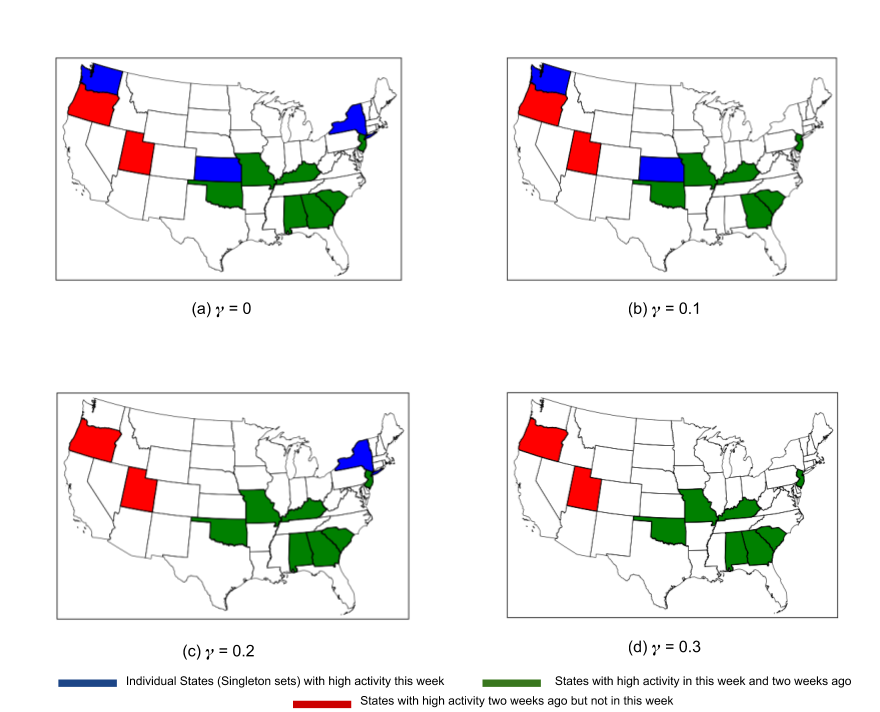
\includegraphics[scale = 0.5]{./figures/relax.png}
\caption{
Effect of $\gamma$ on the description of the set of states which high activity level
in the week of 2017-01-21. 
The states colored green or red had high activity level two weeks ago.
The states colored green or blue (New York, Kansas, Washington) 
in (a) are the ones with high activity level in the current week.
In (b), $\gamma=0.1$, and one blue colored state is dropped.
Panel (c) corresponds to $\gamma=0.2$, and two blue colored states are dropped and the one dropped in (b) is added.
Panel (d) corresponds to $\gamma=0.3$, and the remaining blue state is also dropped.
For $\gamma=0.3$, the description only involves the green and red states.
%%%increasing relaxation parameter from 0 to 0.3 by a step of 0.1 for describing set of states with high during 2017-01-21. Each color represents a set. The green color represents the set of states with high two weeks ago, while red color represents the two states that are excluded from this set. Blue is used for the singleton sets $\{New\;York\}$, $\{Kansas\}$ and $\{Washington\}$. All the states that are colored are part of our target set excluding the ones in red.
}
\label{fig:relaxeffect}
\end{figure}

\subsection*{4. Effect of negative clauses on descriptions}
Some of the descriptions in Table \ref{highactivity} exclude certain states or sets of states. 
This is the result of our target set representation as unions and differences of clauses. 
For instance, in row 5, for $\gamma=0.3$, most states which had a high activity level 
a week ago, except for Wyoming, are at a high activity level currently.
In row 9, the description excludes Florida and Georgia. Such negative clauses
make the descriptions much simpler.
%%%consists of a negative clause containing union of two singleton sets \{Florida\} and \{Georgia\}. The use of negative clauses seems to be useful to give simpler descriptions. For example, it would be easier to comprehend that all south east states are experiencing high activity excluding Georgia, rather than comprehending the list of all those states.




\subsection*{5. Generation of descriptions by ranked order}
%%Ranked Order Descriptions
It is not known a priori which target sets would give interesting patterns.
As discussed earlier, our automated procedure explores a large set of ``potential'' target sets
corresponding to all clauses with up to $k$ terms. We then consider a subset of these, which have
descriptions of low cost, and rank them based on the potential interest for public health.
We assign a score for each type of set, and construct a ranking based on the scores.
Sets consisting of states with high activity level are likely to be more interesting
than those with moderate, low or minimal activity levels;
therefore, these are assigned scores 4, 3, 2, 1 respectively (i.e., 4 for sets with 
high activity level, and so on).
Next, states exhibiting a sudden change in activity level (e.g., from low to high, or vice versa)
are more interesting than those having no change in activity levels;
we assign a score of 5 for the former type, and 2 for the latter.
Then, ``a set of states with high this week and minimal 1 week ago'' has a score of 9, 
while ``a set of states with minimal this week and minimal 1 week ago'' has a score of 3. 
Table \ref{rankedorder} presents the top two scored descriptions for two different weeks,
when run with different parameter settings. 
We find that the top scoring narratives generally are trends, which will be discussed next.


%%%Since our algorithm could generate descriptions for many target sets for each week, it is useful to order these descriptions based on some score of interestingness. For example, describing set of states with high activity could be more useful than describing those with minimal activity. Therefore, the scores for describing the sets of high, moderate, low and minimal activities could be decreasing in that order. Also, it might be useful to describe sets where there is a sudden change in activity levels from low to high or vice-versa. Therefore, describing these kind of patters could be assigned a higher score than describing sets with no change in activity levels. We have used some such assignment of scores to each description and the descriptions with higher scores are considered of higher rank. Below is an example to illustrate this idea:
%%%Example: Let describing sets with high, moderate, low and minimal activities have scores 4, 3, 2, 1 respectively. Also, describing sets with sudden change in activity levels from high to minimal (or vice-versa) within a week be of score 5 and a no change in activity levels is of score 2. Then,``describing a set of states with high this week and minimal 1 week ago'' has a score of 9, while ``describing a set of states with minimal this week and minimal 1 week ago'' has a score of 3. Table \ref{rankedorder} presents the top two scoring narratives for two different weeks run with different parameter settings. The results show that the top scoring narratives generally are trends, which will be discussed in the following section. 


\begin{table}[ht!]
\begin{center}
\begin{tabular}{ | p {1cm} |p {1.8cm} |p {1.7cm} |p {4 cm} | p {4 cm} | p {1.3cm} | } 
\hline
& \textbf{Week} & $(\gamma, \alpha, \beta)$ & \textbf{Target Set} & \textbf{Description} & \textbf{Score} \\ \hline
\multirow{2}{*} 1 &  {2018-01-27} & (0, 2, 2) 
& States with high activity this week(4), low activity two weeks ago (high to low: 5), and moderate three weeks ago (low to moderate: 5)& HI, MD, NC, and OH & 14 \\ \cline{3-6}
& & & States with moderate activity a week ago (3), minimal activity two weeks ago(moderate to minimal:5), and low three weeks ago(moderate to low: 5) & ND & 13 \\ \hline
\multirow{2}{*} 2 &  {2017-02-25} & (0.3, 2, 4) & States with high activity this week(4), low activity a week ago (high to low: 5), moderate two weeks ago (low to moderate: 5) & IA & 14 \\ \cline{3-6}
& & & States with high activity this week (4) and low two weeks ago (high to low: 5)&  MD and MN & 9 \\ 
\hline
\end{tabular}
\caption{Table showing descriptions for two weeks with their scores.}
\label{rankedorder}
\end{center}
\end{table}


\subsection*{6. Trends}
We say that a set of states has a ``trend'' if it exhibits a gradual increase or decrease in 
activity level. Examples of trend type of descriptions found by our method are:
%%The trends are the patterns that are generated by our algorithm. A typical trend in the context of ILI activity levels is a gradual increase in activity in particular set of states. Our results show the inherent patterns in the data and present them succinctly. All the trends are obtained by setting the parameters to the default $(r, p, n) = (0, 2, 2)$. 

\begin{enumerate}
\item \emph{Gradual increase in the activity levels over consecutive weeks}: 
The states AL, GA, MS, and TN
had high activity in the week of 2016-03-12, 
moderate the previous week, and minimal two weeks ago.
%%we present our narrative to describe the set of states with high activity that had moderate activity a week ago and minimal activity three weeks ago respectively. Our narration is as follows: ``Alabama, Georgia, Mississippi and Tennessee''. 
\item \emph{Stable high activity for consecutive weeks}: 
In the week ending 2018-01-27,
the states NJ, NM, VA, WA, WY, and the states 
with high activity four weeks earlier, excluding NE and TN, 
had high activity levels for three consecutive weeks.

%%For the week 2018-01-27, we describe the states with high activity levels since three weeks ago as follows: ``New Jersey, New Mexico, Virginia, Washington,  Wyoming and states with high activity four weeks ago excluding Nebraska and Tennessee''. 
\item \emph{Gradual decrease in ILI activity over consecutive weeks}: 
For the week of 2014-02-01, the activity levels in NC 
decreased from high to moderate to low in three consecutive weeks.
\end{enumerate}

\subsection*{7. Surprises}
We refer to a sudden rise or drop in activity levels (by at least two levels, say, from high to low, moderate to minimal, etc.) within a week's time as a surprise.
Examples of surprise events identified by our methods are:
%%The surprises are a special category of trends where a state experiences sudden rise or drop in activity levels within a week's time. These kinds of surprises are captured well by our narratives. Below we provide some sample results: 
\begin{enumerate}
\item 
The activity level in NC, NM, SD, and WY jumped from
low to high within a week, for the week ending 2017-02-04.
%%Low to High in a week: For the week 2017-02-04, we describe the states with change of activity from low to high within a week as follows: "North Carolina, New Mexico, South Dakota and Wyoming". 
\item 
The activity level in NH and TN changed from high to low within a week,
for the week ending 2013-02-02.
%%High to Low in a week: For the week 2013-02-02, we describe the states with change of activity from high to low within a week as follows: "New Hampshire and Tennessee".
\end{enumerate}
